\section{TunnelEntry}\label{sec:tunent}

\begin{figure}
\begin{center}
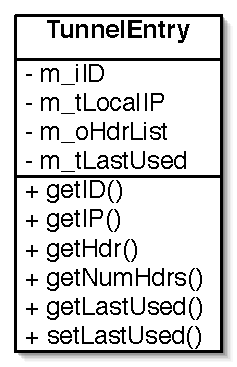
\includegraphics[width=0.4\textwidth]{figs/tunent}
\end{center}
\caption{}
\label{fig:tunent}
\end{figure}

This section describes the TunnelEntry component, which is described by Figure~\ref{fig:tunent}.  This is a very simple abstract data type
(ADT).  It encapsulates the set of headers needed to encapsulate an outbound IP packet, and the local address used to deliver traffic to a
local client.  The goal of this class is to simple wrap the logic that determines how many headers (i.e. levels of NAT) are needed and to
actually encapsulate and de-encapsulate packets.


\subsection{Methods}

{\bf Public Methods}
\begin{itemize}
\item getID(): Simple accessor that returns the ID of this entry.
\item getIP(): Simple accessor that returns the local IP address that corresponds to this tunnel.
\item getHdr(): Takes an ordinal postion and returns the header there.
\item getNumHdrs(): Returns the number of headers.
\item getLastUsed(): Returns the time of the last access.
\item setLastUsed(): Sets the last access time.
\end{itemize}

\subsection{Member Variables}
\begin{itemize}
\item m\_iID: int - Internal ID of this entry.
%\item m\_iFD: int - File descriptor
\item m\_uLocalIP: unit32\_t - Local IP address of this tunnel.
\item m\_oHdrList: list<> - List of headers to enapsulate packets for this tunnel.
\item m\_tLastUsed: time\_t - Time of last use.
\end{itemize}
